\documentclass[twoside]{book}

% Packages required by doxygen
\usepackage{fixltx2e}
\usepackage{calc}
\usepackage{doxygen}
\usepackage[export]{adjustbox} % also loads graphicx
\usepackage{graphicx}
\usepackage[utf8]{inputenc}
\usepackage{makeidx}
\usepackage{multicol}
\usepackage{multirow}
\PassOptionsToPackage{warn}{textcomp}
\usepackage{textcomp}
\usepackage[nointegrals]{wasysym}
\usepackage[table]{xcolor}

% Font selection
\usepackage[T1]{fontenc}
\usepackage[scaled=.90]{helvet}
\usepackage{courier}
\usepackage{amssymb}
\usepackage{sectsty}
\renewcommand{\familydefault}{\sfdefault}
\allsectionsfont{%
  \fontseries{bc}\selectfont%
  \color{darkgray}%
}
\renewcommand{\DoxyLabelFont}{%
  \fontseries{bc}\selectfont%
  \color{darkgray}%
}
\newcommand{\+}{\discretionary{\mbox{\scriptsize$\hookleftarrow$}}{}{}}

% Page & text layout
\usepackage{geometry}
\geometry{%
  a4paper,%
  top=2.5cm,%
  bottom=2.5cm,%
  left=2.5cm,%
  right=2.5cm%
}
\tolerance=750
\hfuzz=15pt
\hbadness=750
\setlength{\emergencystretch}{15pt}
\setlength{\parindent}{0cm}
\setlength{\parskip}{3ex plus 2ex minus 2ex}
\makeatletter
\renewcommand{\paragraph}{%
  \@startsection{paragraph}{4}{0ex}{-1.0ex}{1.0ex}{%
    \normalfont\normalsize\bfseries\SS@parafont%
  }%
}
\renewcommand{\subparagraph}{%
  \@startsection{subparagraph}{5}{0ex}{-1.0ex}{1.0ex}{%
    \normalfont\normalsize\bfseries\SS@subparafont%
  }%
}
\makeatother

% Headers & footers
\usepackage{fancyhdr}
\pagestyle{fancyplain}
\fancyhead[LE]{\fancyplain{}{\bfseries\thepage}}
\fancyhead[CE]{\fancyplain{}{}}
\fancyhead[RE]{\fancyplain{}{\bfseries\leftmark}}
\fancyhead[LO]{\fancyplain{}{\bfseries\rightmark}}
\fancyhead[CO]{\fancyplain{}{}}
\fancyhead[RO]{\fancyplain{}{\bfseries\thepage}}
\fancyfoot[LE]{\fancyplain{}{}}
\fancyfoot[CE]{\fancyplain{}{}}
\fancyfoot[RE]{\fancyplain{}{\bfseries\scriptsize Generated by Doxygen }}
\fancyfoot[LO]{\fancyplain{}{\bfseries\scriptsize Generated by Doxygen }}
\fancyfoot[CO]{\fancyplain{}{}}
\fancyfoot[RO]{\fancyplain{}{}}
\renewcommand{\footrulewidth}{0.4pt}
\renewcommand{\chaptermark}[1]{%
  \markboth{#1}{}%
}
\renewcommand{\sectionmark}[1]{%
  \markright{\thesection\ #1}%
}

% Indices & bibliography
\usepackage{natbib}
\usepackage[titles]{tocloft}
\setcounter{tocdepth}{3}
\setcounter{secnumdepth}{5}
\makeindex

% Hyperlinks (required, but should be loaded last)
\usepackage{ifpdf}
\ifpdf
  \usepackage[pdftex,pagebackref=true]{hyperref}
\else
  \usepackage[ps2pdf,pagebackref=true]{hyperref}
\fi
\hypersetup{%
  colorlinks=true,%
  linkcolor=blue,%
  citecolor=blue,%
  unicode%
}

% Custom commands
\newcommand{\clearemptydoublepage}{%
  \newpage{\pagestyle{empty}\cleardoublepage}%
}

\usepackage{caption}
\captionsetup{labelsep=space,justification=centering,font={bf},singlelinecheck=off,skip=4pt,position=top}

%===== C O N T E N T S =====

\begin{document}

% Titlepage & ToC
\hypersetup{pageanchor=false,
             bookmarksnumbered=true,
             pdfencoding=unicode
            }
\pagenumbering{roman}
\begin{titlepage}
\vspace*{7cm}
\begin{center}%
{\Large My Project }\\
\vspace*{1cm}
{\large Generated by Doxygen 1.8.11}\\
\end{center}
\end{titlepage}
\clearemptydoublepage
\tableofcontents
\clearemptydoublepage
\pagenumbering{arabic}
\hypersetup{pageanchor=true}

%--- Begin generated contents ---
\chapter{Hierarchical Index}
\section{Class Hierarchy}
This inheritance list is sorted roughly, but not completely, alphabetically\+:\begin{DoxyCompactList}
\item \contentsline{section}{Fruit}{\pageref{classFruit}}{}
\begin{DoxyCompactList}
\item \contentsline{section}{Apple}{\pageref{classApple}}{}
\item \contentsline{section}{Grape}{\pageref{classGrape}}{}
\item \contentsline{section}{Orange}{\pageref{classOrange}}{}
\end{DoxyCompactList}
\item \contentsline{section}{List}{\pageref{classList}}{}
\item \contentsline{section}{List\+:\+:Node}{\pageref{structList_1_1Node}}{}
\end{DoxyCompactList}

\chapter{Class Index}
\section{Class List}
Here are the classes, structs, unions and interfaces with brief descriptions\+:\begin{DoxyCompactList}
\item\contentsline{section}{\hyperlink{structnode}{node} }{\pageref{structnode}}{}
\item\contentsline{section}{\hyperlink{structnode1}{node1} }{\pageref{structnode1}}{}
\item\contentsline{section}{\hyperlink{structnode__info}{node\+\_\+info} }{\pageref{structnode__info}}{}
\end{DoxyCompactList}

\chapter{File Index}
\section{File List}
Here is a list of all files with brief descriptions\+:\begin{DoxyCompactList}
\item\contentsline{section}{\hyperlink{Lab1_8c}{Lab1.\+c} }{\pageref{Lab1_8c}}{}
\end{DoxyCompactList}

\chapter{Class Documentation}
\hypertarget{classbase1}{}\section{base1 Class Reference}
\label{classbase1}\index{base1@{base1}}


Inheritance diagram for base1\+:
\nopagebreak
\begin{figure}[H]
\begin{center}
\leavevmode
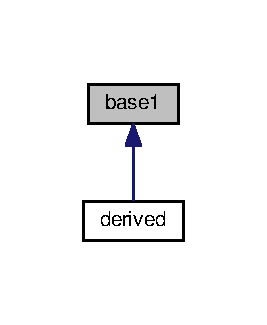
\includegraphics[width=128pt]{classbase1__inherit__graph}
\end{center}
\end{figure}
\subsection*{Public Member Functions}
\begin{DoxyCompactItemize}
\item 
\hyperlink{classbase1_a7a9c58df41f166a95af8c65fe67e2f60}{base1} (int x)
\item 
\hyperlink{classbase1_a0d95fcd85fda77d8cf761b1aa56336ad}{$\sim$base1} ()
\end{DoxyCompactItemize}
\subsection*{Protected Attributes}
\begin{DoxyCompactItemize}
\item 
int \hyperlink{classbase1_adf92d07b7fc0fe0c61b2a42f5ebe0f88}{i}
\end{DoxyCompactItemize}


\subsection{Constructor \& Destructor Documentation}
\index{base1@{base1}!base1@{base1}}
\index{base1@{base1}!base1@{base1}}
\subsubsection[{\texorpdfstring{base1(int x)}{base1(int x)}}]{\setlength{\rightskip}{0pt plus 5cm}base1\+::base1 (
\begin{DoxyParamCaption}
\item[{int}]{x}
\end{DoxyParamCaption}
)\hspace{0.3cm}{\ttfamily [inline]}}\hypertarget{classbase1_a7a9c58df41f166a95af8c65fe67e2f60}{}\label{classbase1_a7a9c58df41f166a95af8c65fe67e2f60}

\begin{DoxyCode}
8 \{ \hyperlink{classbase1_adf92d07b7fc0fe0c61b2a42f5ebe0f88}{i} = x; cout << \textcolor{stringliteral}{"Constructing base1\(\backslash\)n"}; \}
\end{DoxyCode}
\index{base1@{base1}!````~base1@{$\sim$base1}}
\index{````~base1@{$\sim$base1}!base1@{base1}}
\subsubsection[{\texorpdfstring{$\sim$base1()}{~base1()}}]{\setlength{\rightskip}{0pt plus 5cm}base1\+::$\sim$base1 (
\begin{DoxyParamCaption}
{}
\end{DoxyParamCaption}
)\hspace{0.3cm}{\ttfamily [inline]}}\hypertarget{classbase1_a0d95fcd85fda77d8cf761b1aa56336ad}{}\label{classbase1_a0d95fcd85fda77d8cf761b1aa56336ad}

\begin{DoxyCode}
9 \{ cout << \textcolor{stringliteral}{"Destructing base2\(\backslash\)n"}; \}
\end{DoxyCode}


\subsection{Member Data Documentation}
\index{base1@{base1}!i@{i}}
\index{i@{i}!base1@{base1}}
\subsubsection[{\texorpdfstring{i}{i}}]{\setlength{\rightskip}{0pt plus 5cm}int base1\+::i\hspace{0.3cm}{\ttfamily [protected]}}\hypertarget{classbase1_adf92d07b7fc0fe0c61b2a42f5ebe0f88}{}\label{classbase1_adf92d07b7fc0fe0c61b2a42f5ebe0f88}


The documentation for this class was generated from the following file\+:\begin{DoxyCompactItemize}
\item 
\hyperlink{Inheritance_8cpp}{Inheritance.\+cpp}\end{DoxyCompactItemize}

\hypertarget{classbase2}{}\section{base2 Class Reference}
\label{classbase2}\index{base2@{base2}}


Inheritance diagram for base2\+:
\nopagebreak
\begin{figure}[H]
\begin{center}
\leavevmode
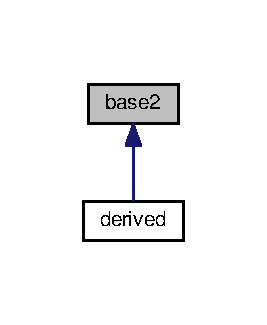
\includegraphics[width=128pt]{classbase2__inherit__graph}
\end{center}
\end{figure}
\subsection*{Public Member Functions}
\begin{DoxyCompactItemize}
\item 
\hyperlink{classbase2_a803b52718de7ad0a819aa35af24bfb0b}{base2} (int x)
\item 
\hyperlink{classbase2_acedaa55eb8c7a90c93e814267b228762}{$\sim$base2} ()
\end{DoxyCompactItemize}
\subsection*{Protected Attributes}
\begin{DoxyCompactItemize}
\item 
int \hyperlink{classbase2_a5edebd513b4b4aaba4907d040b2f38ce}{k}
\end{DoxyCompactItemize}


\subsection{Constructor \& Destructor Documentation}
\index{base2@{base2}!base2@{base2}}
\index{base2@{base2}!base2@{base2}}
\subsubsection[{\texorpdfstring{base2(int x)}{base2(int x)}}]{\setlength{\rightskip}{0pt plus 5cm}base2\+::base2 (
\begin{DoxyParamCaption}
\item[{int}]{x}
\end{DoxyParamCaption}
)\hspace{0.3cm}{\ttfamily [inline]}}\hypertarget{classbase2_a803b52718de7ad0a819aa35af24bfb0b}{}\label{classbase2_a803b52718de7ad0a819aa35af24bfb0b}

\begin{DoxyCode}
16 \{ \hyperlink{classbase2_a5edebd513b4b4aaba4907d040b2f38ce}{k} = x; cout << \textcolor{stringliteral}{"Constructing base2\(\backslash\)n"}; \}
\end{DoxyCode}
\index{base2@{base2}!````~base2@{$\sim$base2}}
\index{````~base2@{$\sim$base2}!base2@{base2}}
\subsubsection[{\texorpdfstring{$\sim$base2()}{~base2()}}]{\setlength{\rightskip}{0pt plus 5cm}base2\+::$\sim$base2 (
\begin{DoxyParamCaption}
{}
\end{DoxyParamCaption}
)\hspace{0.3cm}{\ttfamily [inline]}}\hypertarget{classbase2_acedaa55eb8c7a90c93e814267b228762}{}\label{classbase2_acedaa55eb8c7a90c93e814267b228762}

\begin{DoxyCode}
17 \{ cout << \textcolor{stringliteral}{"Destructing base2\(\backslash\)n"}; \}
\end{DoxyCode}


\subsection{Member Data Documentation}
\index{base2@{base2}!k@{k}}
\index{k@{k}!base2@{base2}}
\subsubsection[{\texorpdfstring{k}{k}}]{\setlength{\rightskip}{0pt plus 5cm}int base2\+::k\hspace{0.3cm}{\ttfamily [protected]}}\hypertarget{classbase2_a5edebd513b4b4aaba4907d040b2f38ce}{}\label{classbase2_a5edebd513b4b4aaba4907d040b2f38ce}


The documentation for this class was generated from the following file\+:\begin{DoxyCompactItemize}
\item 
\hyperlink{Inheritance_8cpp}{Inheritance.\+cpp}\end{DoxyCompactItemize}

\hypertarget{classderived}{}\section{derived Class Reference}
\label{classderived}\index{derived@{derived}}


Inheritance diagram for derived\+:
\nopagebreak
\begin{figure}[H]
\begin{center}
\leavevmode
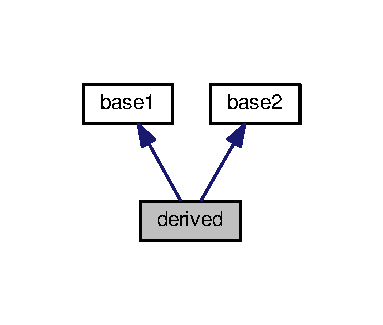
\includegraphics[width=184pt]{classderived__inherit__graph}
\end{center}
\end{figure}


Collaboration diagram for derived\+:
\nopagebreak
\begin{figure}[H]
\begin{center}
\leavevmode
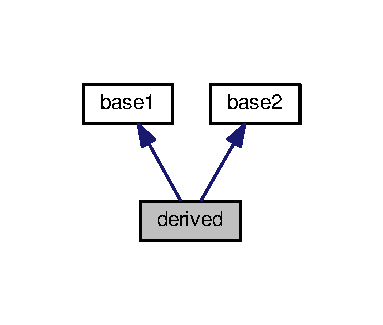
\includegraphics[width=184pt]{classderived__coll__graph}
\end{center}
\end{figure}
\subsection*{Public Member Functions}
\begin{DoxyCompactItemize}
\item 
\hyperlink{classderived_a187a2a11010dbded8bc498cb65ccb47d}{derived} (int x, int y, int z)
\item 
\hyperlink{classderived_a6d07faec327a1108a1a78f4585689e1c}{$\sim$derived} ()
\item 
void \hyperlink{classderived_aadf177f8b84402f519c92072dab5a89b}{show} ()
\end{DoxyCompactItemize}
\subsection*{Private Attributes}
\begin{DoxyCompactItemize}
\item 
int \hyperlink{classderived_a185f22d57af96279b433efaab36aeac3}{j}
\end{DoxyCompactItemize}
\subsection*{Additional Inherited Members}


\subsection{Constructor \& Destructor Documentation}
\index{derived@{derived}!derived@{derived}}
\index{derived@{derived}!derived@{derived}}
\subsubsection[{\texorpdfstring{derived(int x, int y, int z)}{derived(int x, int y, int z)}}]{\setlength{\rightskip}{0pt plus 5cm}derived\+::derived (
\begin{DoxyParamCaption}
\item[{int}]{x, }
\item[{int}]{y, }
\item[{int}]{z}
\end{DoxyParamCaption}
)\hspace{0.3cm}{\ttfamily [inline]}}\hypertarget{classderived_a187a2a11010dbded8bc498cb65ccb47d}{}\label{classderived_a187a2a11010dbded8bc498cb65ccb47d}

\begin{DoxyCode}
23                               : \hyperlink{classbase1_a7a9c58df41f166a95af8c65fe67e2f60}{base1}(y), \hyperlink{classbase2_a803b52718de7ad0a819aa35af24bfb0b}{base2}(z)
24     \{ \hyperlink{classderived_a185f22d57af96279b433efaab36aeac3}{j} = x; cout << \textcolor{stringliteral}{"Constructing derived\(\backslash\)n"}; \}
\end{DoxyCode}
\index{derived@{derived}!````~derived@{$\sim$derived}}
\index{````~derived@{$\sim$derived}!derived@{derived}}
\subsubsection[{\texorpdfstring{$\sim$derived()}{~derived()}}]{\setlength{\rightskip}{0pt plus 5cm}derived\+::$\sim$derived (
\begin{DoxyParamCaption}
{}
\end{DoxyParamCaption}
)\hspace{0.3cm}{\ttfamily [inline]}}\hypertarget{classderived_a6d07faec327a1108a1a78f4585689e1c}{}\label{classderived_a6d07faec327a1108a1a78f4585689e1c}

\begin{DoxyCode}
26 \{ cout << \textcolor{stringliteral}{"Destructing derived\(\backslash\)n"}; \}
\end{DoxyCode}


\subsection{Member Function Documentation}
\index{derived@{derived}!show@{show}}
\index{show@{show}!derived@{derived}}
\subsubsection[{\texorpdfstring{show()}{show()}}]{\setlength{\rightskip}{0pt plus 5cm}void derived\+::show (
\begin{DoxyParamCaption}
{}
\end{DoxyParamCaption}
)\hspace{0.3cm}{\ttfamily [inline]}}\hypertarget{classderived_aadf177f8b84402f519c92072dab5a89b}{}\label{classderived_aadf177f8b84402f519c92072dab5a89b}

\begin{DoxyCode}
27 \{ cout << \hyperlink{classbase1_adf92d07b7fc0fe0c61b2a42f5ebe0f88}{i} << \textcolor{stringliteral}{" "} << \hyperlink{classderived_a185f22d57af96279b433efaab36aeac3}{j} << \textcolor{stringliteral}{" "} << \hyperlink{classbase2_a5edebd513b4b4aaba4907d040b2f38ce}{k} << \textcolor{stringliteral}{"\(\backslash\)n"}; \}
\end{DoxyCode}


\subsection{Member Data Documentation}
\index{derived@{derived}!j@{j}}
\index{j@{j}!derived@{derived}}
\subsubsection[{\texorpdfstring{j}{j}}]{\setlength{\rightskip}{0pt plus 5cm}int derived\+::j\hspace{0.3cm}{\ttfamily [private]}}\hypertarget{classderived_a185f22d57af96279b433efaab36aeac3}{}\label{classderived_a185f22d57af96279b433efaab36aeac3}


The documentation for this class was generated from the following file\+:\begin{DoxyCompactItemize}
\item 
\hyperlink{Inheritance_8cpp}{Inheritance.\+cpp}\end{DoxyCompactItemize}

\chapter{File Documentation}
\hypertarget{Inheritance_8cpp}{}\section{Inheritance.\+cpp File Reference}
\label{Inheritance_8cpp}\index{Inheritance.\+cpp@{Inheritance.\+cpp}}
{\ttfamily \#include $<$iostream$>$}\\*
Include dependency graph for Inheritance.\+cpp\+:
\nopagebreak
\begin{figure}[H]
\begin{center}
\leavevmode
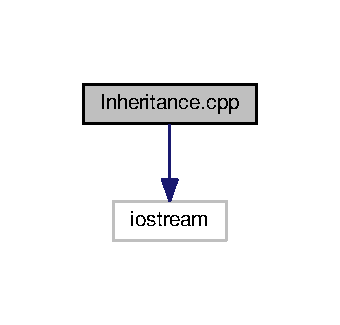
\includegraphics[width=163pt]{Inheritance_8cpp__incl}
\end{center}
\end{figure}
\subsection*{Classes}
\begin{DoxyCompactItemize}
\item 
class \hyperlink{classbase1}{base1}
\item 
class \hyperlink{classbase2}{base2}
\item 
class \hyperlink{classderived}{derived}
\end{DoxyCompactItemize}
\subsection*{Functions}
\begin{DoxyCompactItemize}
\item 
int \hyperlink{Inheritance_8cpp_ae66f6b31b5ad750f1fe042a706a4e3d4}{main} ()
\end{DoxyCompactItemize}


\subsection{Function Documentation}
\index{Inheritance.\+cpp@{Inheritance.\+cpp}!main@{main}}
\index{main@{main}!Inheritance.\+cpp@{Inheritance.\+cpp}}
\subsubsection[{\texorpdfstring{main()}{main()}}]{\setlength{\rightskip}{0pt plus 5cm}int main (
\begin{DoxyParamCaption}
{}
\end{DoxyParamCaption}
)}\hypertarget{Inheritance_8cpp_ae66f6b31b5ad750f1fe042a706a4e3d4}{}\label{Inheritance_8cpp_ae66f6b31b5ad750f1fe042a706a4e3d4}

\begin{DoxyCode}
31 \{
32   \hyperlink{classderived}{derived} ob(3, 4, 5);
33 
34   ob.show();  \textcolor{comment}{// displays 4 3 5}
35 
36   \textcolor{keywordflow}{return} 0;
37 \}
\end{DoxyCode}


Here is the call graph for this function\+:
\nopagebreak
\begin{figure}[H]
\begin{center}
\leavevmode
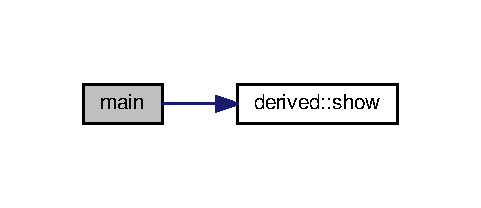
\includegraphics[width=231pt]{Inheritance_8cpp_ae66f6b31b5ad750f1fe042a706a4e3d4_cgraph}
\end{center}
\end{figure}



%--- End generated contents ---

% Index
\backmatter
\newpage
\phantomsection
\clearemptydoublepage
\addcontentsline{toc}{chapter}{Index}
\printindex

\end{document}
